\hypertarget{section-better-proof-tools}{%
\section{Section: Better proof tools}\label{section-better-proof-tools}}

\interlude*<left,leftskip=7cm,>[90]<Tribulations \textasciitilde\ Tooling>{Oh These\\Proof Tools}<Vive la Révolution! Against the Bourgeoisie of Proof Assistants!>

\begin{frame}{In the following slides, you will hear…}

  %$\dots$ and mechanised proofs have not covered this thus far.

  %\vspace{5em}

  \blockquote[Helen Keller (1880-1968) in The Day Language Came into My Life]{
    Everything had a name, and each name gave birth to a new thought.
  }

% We do not want to be typecast into people who just do usability or accessibility

% language creates awareness, consciousness

% neces. prerequisite 

% in order to be able to reason mathematically

% math is the process of giving, of express math
% concepts in the form of language
% 

% math is something fundamentally kommunikatives

% that's an aspect that mechanised proofs haven't covered thus far

% Everything had a name, and each name gave birth to a new thought.
% --- Helen Keller (1880-1968) in The Day Language Came into My Life


% https://www.pval.org/cms/lib/NY19000481/Centricity/Domain/105/The%20Day%20Language%20Came%20into%20my%20Life.pdf

\end{frame}



\begin{frame}{Symbolic Modeling of Rosenpass}
\hypertarget{analysis-usability-colorful-proverif-voice}{}
  \begin{columns}[c]
    \begin{column}{.5\linewidth}
     \rlap{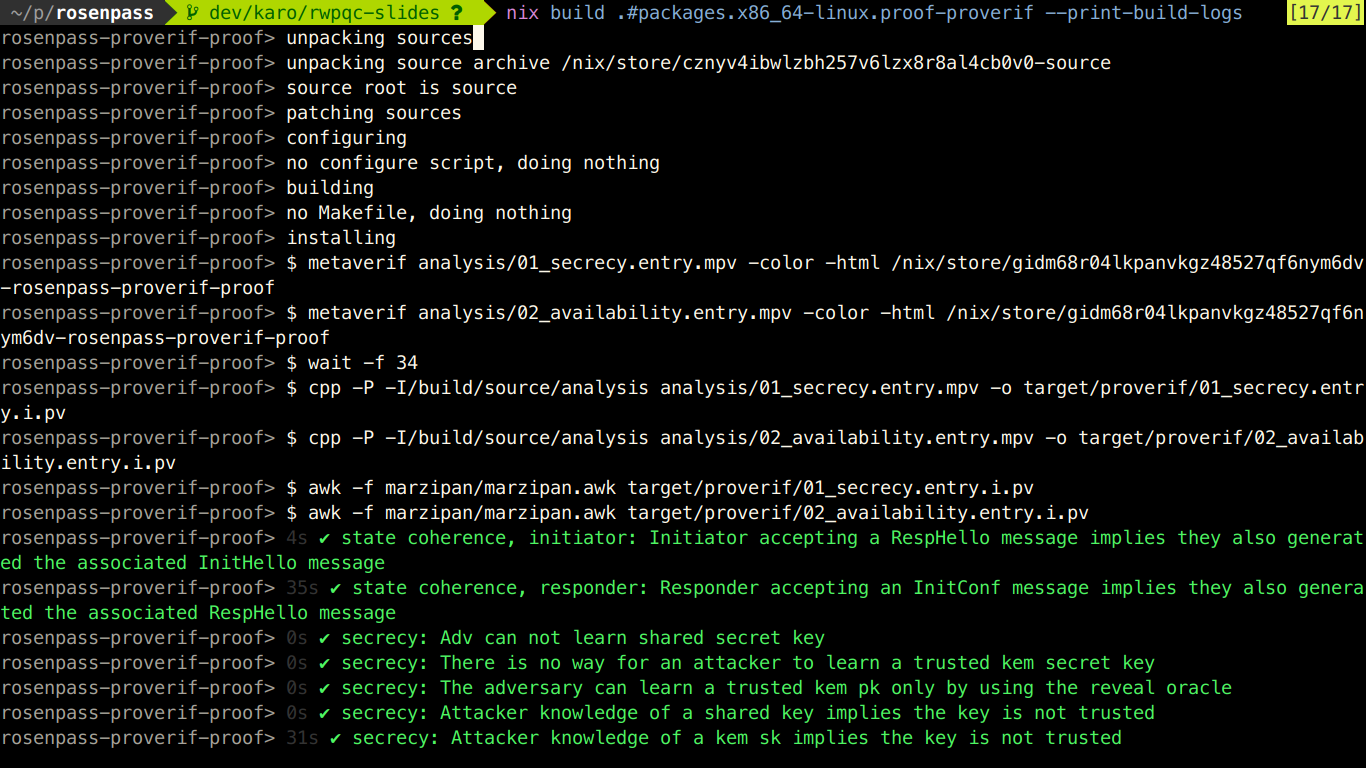
\includegraphics[keepaspectratio,height=.85\textheight]{graphics/2023-03-20-symbolic-analysis-screenshot.png}}
    \end{column}

	  %\pause

    \begin{column}{.5\linewidth}
    \tikz\node[rectangle,fill opacity=1,fill=white,minimum height=.85\textheight, text width=\linewidth]{
      \begin{itemize}
        \item Symbolic modeling using ProVerif
        \item Proofs treated as part of the codebase
        \item Uses a model internally that is based on a fairly comprehensive Maximum Exposure Attacks (MEX) variant
        \item Covers non-interruptability (resistance to disruption attacks)
        \item Mechanized proof in the computational model is an open issue
      \end{itemize}};
    \end{column}
  \end{columns}
\end{frame}




\begin{frame}{Problematic Parts of Pen-and-Paper Proofs}
\hypertarget{problematic-proofs}{}
  \begin{columns}[fullwidth,c]
    \begin{column}{.3\linewidth}
      
\includegraphics[width=\linewidth]{graphics/this-is-fine-crop.png}\\
      
\includegraphics[width=\linewidth]{graphics/this-is-not-fine-crop.jpg}%
    \end{column}
    \hspace{1.2em}
    \begin{column}{.68\linewidth}
      \small

      Bellare and Rogaway: [BR06]\\
      \hspace{1.618em} many “essentially unverifiable” proofs, “crisis of rigor”\\[1.5em]

      Halevi: [Hal05]\\
      \hspace{1.618em} some reasons are social, but “our proofs are truly complex”\\[1.5em]

      Joseph Jaeger: [ProTeCS 2024, Workshop at Eurocrypt]\\
      \hspace{1.618em} technical and social reasons
      \hspace{1.618em} why and for whom do we write proofs?\\[1.5em]%

      We'd like to add:\\
      \hspace{1.618em} pen-and-paper proofs are hard to maintain, update, reuse\\
      \hspace{1.618em} especially for 3rd parties\\[1.5em]%

      Can proofs become part of a continuous engineering effort?%
    \end{column}
  \end{columns}
\end{frame}





\begin{frame}{Friction \& Frustration for the Working Cryptographer}
  \hypertarget{friction-frustration}{}
  \textbf{Tooling}
  \begin{itemize}
    \item Syntax highlighting, favorite editor
    \item Engineering for large models: syntax rewriting, syntactic sugar, macros
    \item Comfortable tooling to inspect intermediate games (CryptoVerif)
  \end{itemize}
  \vspace{1em}
  \textbf{Documentation:} Often incomplete; step from example to research too big\\[.8em]

  \textbf{Output:} hard to understand for non-experts\\[.8em]

  \textbf{Input Language:} Unintuitive? Inaccessible? Mixed signals!\\[.8em]

  \textbf{Proof Language:} not enough flexibility and leeway compared to pen-and-paper
  \begin{itemize}
    \item hand-waving, unsafe blocks
      % pen-and-paper get way more leeway, mechanized proofs are often all or nothing
    \item support for incremental process
  \end{itemize}
\end{frame}









\begin{frame}{Rosenpass going Rube-Goldberg}
  \hypertarget{rosenpass-going-rube-goldberg}{}
  \begin{columns}[fullwidth,T]

    \begin{column}{.8\linewidth}
      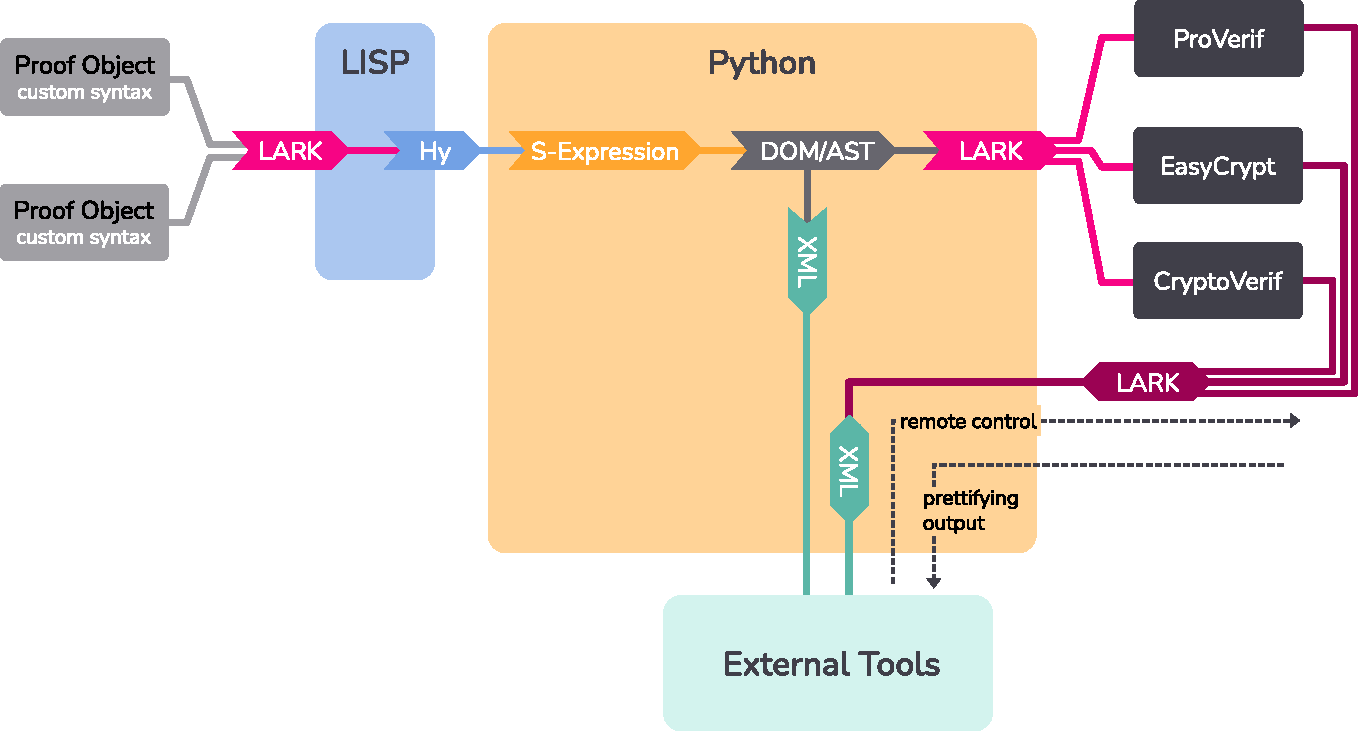
\includegraphics[height=.85\textheight]{graphics/python-proofs.pdf}
    \end{column}

    \begin{column}{.2\linewidth}
      \textbf{Idea:} Build a framework around existing tools
      \medskip

      \textbf{Keep} expressivity and preciseness

      \medskip
      \textbf{Generate and parse} their languages

      \medskip
      \textbf{Open them up} to ecosystems in Python, Lisp, XML
    \end{column}

  \end{columns}
\end{frame}
